% Options for packages loaded elsewhere
\PassOptionsToPackage{unicode}{hyperref}
\PassOptionsToPackage{hyphens}{url}
\documentclass[
  brazilian,
  8pt,
  oneside]{book}
\usepackage{xcolor}
\usepackage[margin=2.2cm]{geometry}
\usepackage{amsmath,amssymb}
\setcounter{secnumdepth}{5}
\usepackage{iftex}
\ifPDFTeX
  \usepackage[T1]{fontenc}
  \usepackage[utf8]{inputenc}
  \usepackage{textcomp} % provide euro and other symbols
\else % if luatex or xetex
  \usepackage{unicode-math} % this also loads fontspec
  \defaultfontfeatures{Scale=MatchLowercase}
  \defaultfontfeatures[\rmfamily]{Ligatures=TeX,Scale=1}
\fi
\usepackage{lmodern}
\ifPDFTeX\else
  % xetex/luatex font selection
\fi
% Use upquote if available, for straight quotes in verbatim environments
\IfFileExists{upquote.sty}{\usepackage{upquote}}{}
\IfFileExists{microtype.sty}{% use microtype if available
  \usepackage[]{microtype}
  \UseMicrotypeSet[protrusion]{basicmath} % disable protrusion for tt fonts
}{}
\makeatletter
\@ifundefined{KOMAClassName}{% if non-KOMA class
  \IfFileExists{parskip.sty}{%
    \usepackage{parskip}
  }{% else
    \setlength{\parindent}{0pt}
    \setlength{\parskip}{6pt plus 2pt minus 1pt}}
}{% if KOMA class
  \KOMAoptions{parskip=half}}
\makeatother
\usepackage{longtable,booktabs,array}
\usepackage{calc} % for calculating minipage widths
% Correct order of tables after \paragraph or \subparagraph
\usepackage{etoolbox}
\makeatletter
\patchcmd\longtable{\par}{\if@noskipsec\mbox{}\fi\par}{}{}
\makeatother
% Allow footnotes in longtable head/foot
\IfFileExists{footnotehyper.sty}{\usepackage{footnotehyper}}{\usepackage{footnote}}
\makesavenoteenv{longtable}
\usepackage{graphicx}
\makeatletter
\newsavebox\pandoc@box
\newcommand*\pandocbounded[1]{% scales image to fit in text height/width
  \sbox\pandoc@box{#1}%
  \Gscale@div\@tempa{\textheight}{\dimexpr\ht\pandoc@box+\dp\pandoc@box\relax}%
  \Gscale@div\@tempb{\linewidth}{\wd\pandoc@box}%
  \ifdim\@tempb\p@<\@tempa\p@\let\@tempa\@tempb\fi% select the smaller of both
  \ifdim\@tempa\p@<\p@\scalebox{\@tempa}{\usebox\pandoc@box}%
  \else\usebox{\pandoc@box}%
  \fi%
}
% Set default figure placement to htbp
\def\fps@figure{htbp}
\makeatother
\ifLuaTeX
\usepackage[bidi=basic]{babel}
\else
\usepackage[bidi=default]{babel}
\fi
% get rid of language-specific shorthands (see #6817):
\let\LanguageShortHands\languageshorthands
\def\languageshorthands#1{}
\setlength{\emergencystretch}{3em} % prevent overfull lines
\providecommand{\tightlist}{%
  \setlength{\itemsep}{0pt}\setlength{\parskip}{0pt}}
\usepackage{bookmark}
\IfFileExists{xurl.sty}{\usepackage{xurl}}{} % add URL line breaks if available
\urlstyle{same}
\hypersetup{
  pdftitle={Garments Planner},
  pdfauthor={Helena Regina Salomé D'Espindula},
  pdflang={pt-BR},
  hidelinks,
  pdfcreator={LaTeX via pandoc}}

\title{Garments Planner}
\author{Helena Regina Salomé D'Espindula}
\date{22/01/2026}

\begin{document}
\maketitle

{
\setcounter{tocdepth}{1}
\tableofcontents
}
\chapter{Classificação de tecidos naturais --- panos e malhas}\label{classificauxe7uxe3o-de-tecidos-naturais-panos-e-malhas}

Placeholder

\chapter{Medidas do corpo}\label{medidas-do-corpo}

Data das medidas: \fieldline

\begin{quote}
Dica: se fizer novas medidas, copie esta pagina e atualize a data.
\end{quote}

\begin{longtable}{p{0.55\linewidth} p{0.15\linewidth} p{0.25\linewidth}}
\toprule
\textbf{Medida} & \textbf{Unid.} & \textbf{Valor} \\
\midrule
\endhead
Ankle circumference & cm & \fieldline \\
Biceps circumference & cm & \fieldline \\
Bust front & cm & \fieldline \\
Bust point to underbust & cm & \fieldline \\
Bust span & cm & \fieldline \\
Chest circumference & cm & \fieldline \\
Cross seam & cm & \fieldline \\
Cross seam front & cm & \fieldline \\
Crotch depth & cm & \fieldline \\
Head circumference & cm & \fieldline \\
Heel circumference & cm & \fieldline \\
High bust & cm & \fieldline \\
High bust front & cm & \fieldline \\
Hips circumference & cm & \fieldline \\
HPS to bust & cm & \fieldline \\
HPS to waist back & cm & \fieldline \\
HPS to waist front & cm & \fieldline \\
Inseam & cm & \fieldline \\
Knee circumference & cm & \fieldline \\
Neck circumference & cm & \fieldline \\
Seat circumference & cm & \fieldline \\
Seat back & cm & \fieldline \\
Shoulder slope & \textdegree & \fieldline \\
Shoulder to elbow & cm & \fieldline \\
Shoulder to shoulder & cm & \fieldline \\
Shoulder to wrist & cm & \fieldline \\
Underbust & cm & \fieldline \\
Upper leg circumference & cm & \fieldline \\
Waist circumference & cm & \fieldline \\
Waist back & cm & \fieldline \\
Waist to armpit & cm & \fieldline \\
Waist to floor & cm & \fieldline \\
Waist to hips & cm & \fieldline \\
Waist to knee & cm & \fieldline \\
Waist to seat & cm & \fieldline \\
Waist to underbust & cm & \fieldline \\
Waist to upper leg & cm & \fieldline \\
Wrist circumference & cm & \fieldline \\
\bottomrule
\end{longtable}

\categorybreak

\chapter{Projetos}\label{projetos}

\begin{quote}
Cada projeto abaixo foi pensado para impressao.\\
Use \texttt{-\/-\/-\/-} como linha separadora entre projetos.
\end{quote}

\section{\texorpdfstring{Projeto: \fieldline}{Projeto: }}\label{projeto}

\subsection{Detalhes do projeto}\label{detalhes-do-projeto}

\begin{itemize}
\tightlist
\item
  Nome do molde / pattern: \fieldline  
\item
  Marca / empresa: \fieldline  
\item
  Tamanho cortado: \fieldline  
\item
  Versao / variacao: \fieldline  
\item
  Data de inicio: \fieldline  
\item
  Data de termino: \fieldline  
\item
  Objetivo (uso, ocasiao, estacao): \fieldline  
\end{itemize}

\subsection{Croqui (frente e costas)}\label{croqui-frente-e-costas}

\begin{center}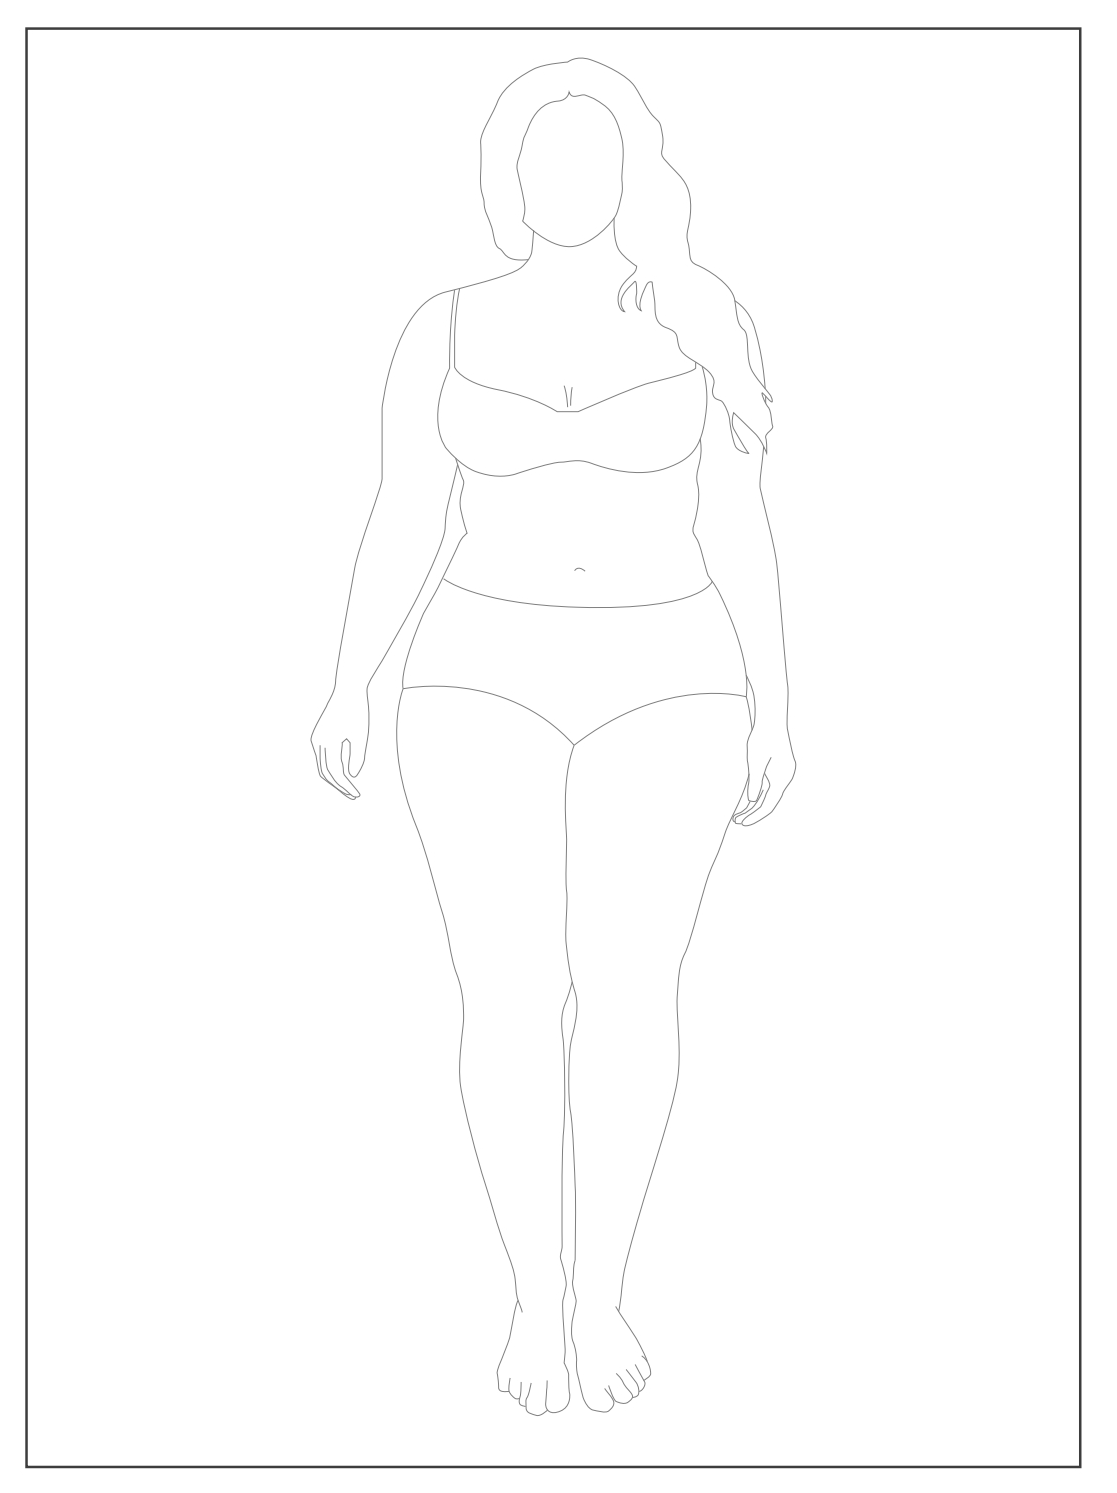
\includegraphics[width=0.48\textwidth]{Croqui_limpo_frente} 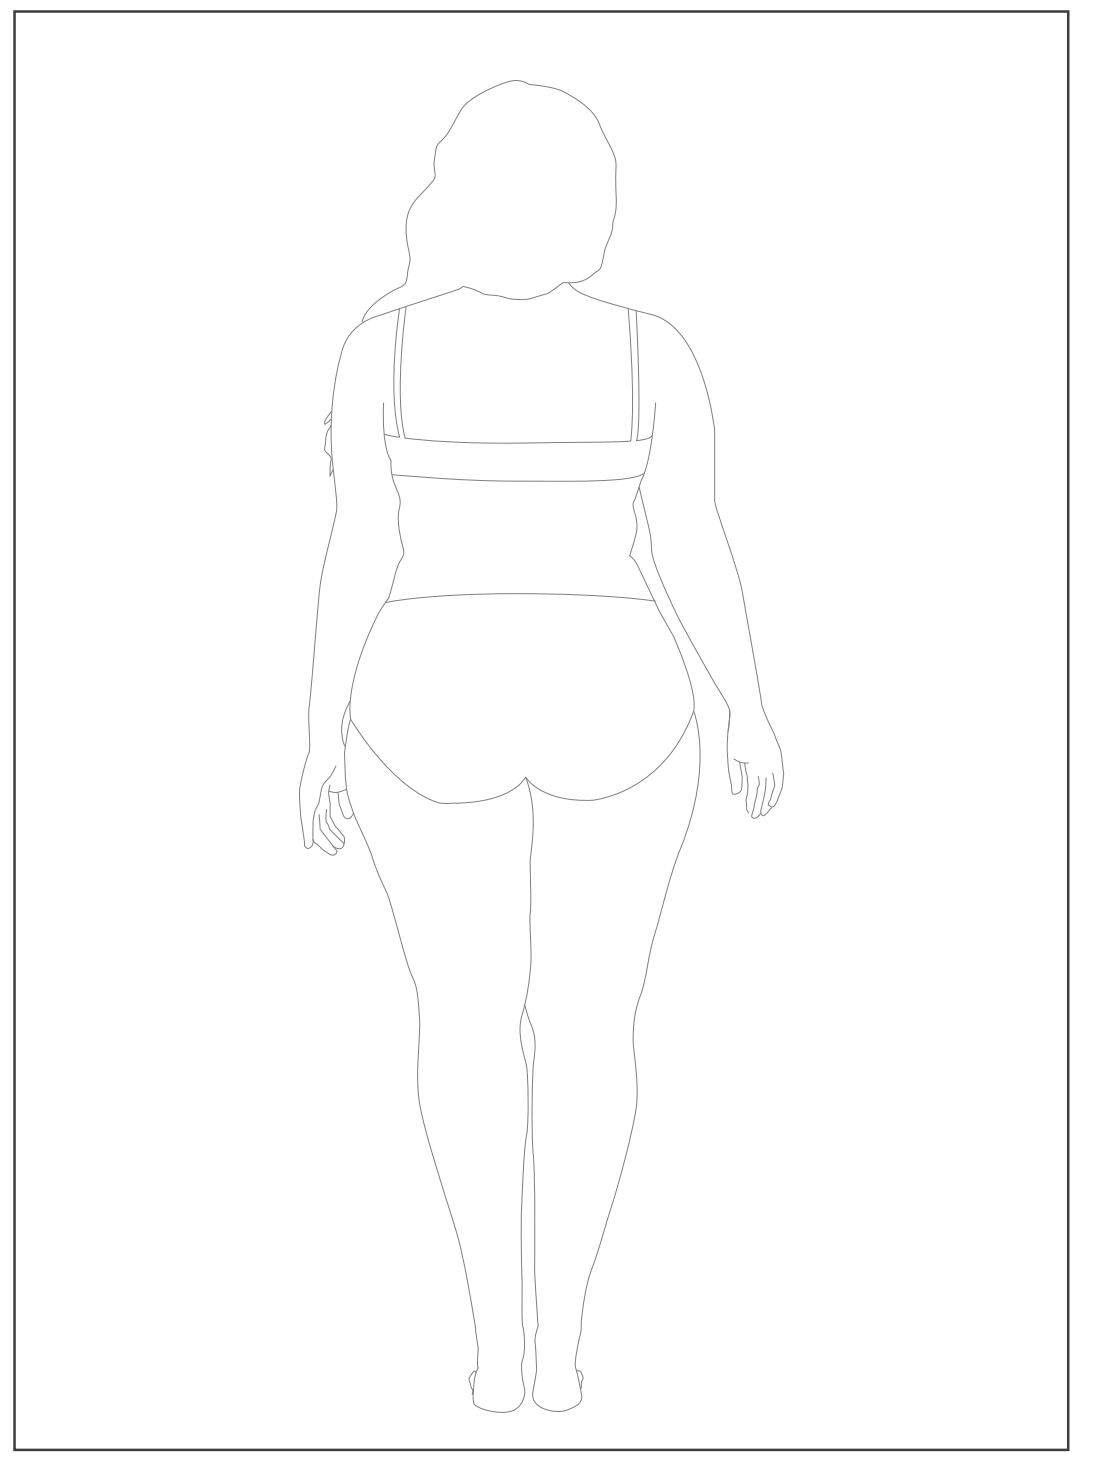
\includegraphics[width=0.48\textwidth]{Croqui_limpo_costas} \end{center}

\subsection{Tecidos usados (espaco para swatches)}\label{tecidos-usados-espaco-para-swatches}

\begin{tabular}{p{0.48\linewidth} p{0.48\linewidth}}
\textbf{Tecido 1} & \textbf{Tecido 2} \\
Fibra: \fieldline & Fibra: \fieldline \\
Origem/loja: \fieldline & Origem/loja: \fieldline \\
Uso no projeto: \fieldline & Uso no projeto: \fieldline \\
\swatchbox & \swatchbox \\
\end{tabular}

\bigskip

\begin{tabular}{p{0.48\linewidth} p{0.48\linewidth}}
\textbf{Tecido 3} & \textbf{Tecido 4} \\
Fibra: \fieldline & Fibra: \fieldline \\
Origem/loja: \fieldline & Origem/loja: \fieldline \\
Uso no projeto: \fieldline & Uso no projeto: \fieldline \\
\swatchbox & \swatchbox \\
\end{tabular}

\subsection{Materiais e aviamentos}\label{materiais-e-aviamentos}

\begin{itemize}
\tightlist
\item
  Linhas: \fieldline  
\item
  Ziper / fechos: \fieldline  
\item
  Botoes: \fieldline  
\item
  Elastico: \fieldline  
\item
  Entretela / interfacing: \fieldline  
\item
  Outros: \fieldline  
\end{itemize}

\subsection{Alteracoes e ajustes}\label{alteracoes-e-ajustes}

\begin{itemize}
\tightlist
\item
  Ajustes no molde: \fieldline  
\end{itemize}

\bigskip
\labelline{Ajustes adicionais}

\bigskip
\labelline{Observacoes de prova}

\subsection{Checklist rapido}\label{checklist-rapido}

\begin{itemize}
\tightlist
\item[$\square$]
  Corte conferido
\item[$\square$]
  Marcas transferidas
\item[$\square$]
  Entretela aplicada (se houver)
\item[$\square$]
  Primeira prova
\item[$\square$]
  Acabamentos internos
\item[$\square$]
  Bainha
\item[$\square$]
  Passadoria final
\end{itemize}

\subsection{Notas e aprendizado}\label{notas-e-aprendizado}

\labelline{O que aprendi / o que faria diferente}

\bigskip
\labelline{Tempo real x tempo estimado}

\begin{longtable}[]{@{}
  >{\raggedright\arraybackslash}p{(\linewidth - 0\tabcolsep) * \real{0.0694}}@{}}
\toprule\noalign{}
\endhead
\bottomrule\noalign{}
\endlastfoot
\#\# Projeto: \\
(duplique o bloco de projeto acima para cada nova peca) \\
\newpage \\
\# Checklist de Costura --- Blusa Simples (G1, tecido leve 100\%) \\
\#\# FASE 0 --- Preparação do tecido \\
- {[} {]} Conferir composição do tecido (100\% natural)
- {[} {]} Verificar se o tecido desfia facilmente \\
\#\#\# Proteção das bordas (antes da lavagem)
- {[} {]} Passar ponto zigue-zague na máquina em \textbf{todas as bordas do pano inteiro}
- {[} {]} Usar ponto zigue-zague largo, sem tensão excessiva
- {[} {]} Não cortar peças antes da lavagem \\
\#\#\# Pré-lavagem
- {[} {]} Dobrar o tecido com cuidado
- {[} {]} Colocar o tecido em \textbf{sacola de lavagem}
- {[} {]} Lavar como a peça será lavada depois (mesma temperatura e sabão)
- {[} {]} Não usar amaciante \\
\#\#\# Secagem e estabilização
- {[} {]} Secar à sombra
- {[} {]} Não torcer o tecido
- {[} {]} Evitar pendurar pelas extremidades
- {[} {]} Passar o tecido após seco
- {[} {]} Alinhar o fio ao passar
- {[} {]} Usar vapor moderado
- {[} {]} Não arrastar o ferro \\
\end{longtable}

\section{FASE 1 --- Modelagem e preparação (papel)}\label{fase-1-modelagem-e-preparauxe7uxe3o-papel}

\begin{itemize}
\tightlist
\item[$\square$]
  Copiar todos os moldes para papel Kraft
\item[$\square$]
  Identificar cada molde (nome da peça, tamanho G1, quantidade de cortes)
\item[$\square$]
  Marcar linha do fio em todas as peças
\item[$\square$]
  Marcar centro da frente
\item[$\square$]
  Marcar centro das costas
\item[$\square$]
  Marcar centro da manga (topo da copa)
\item[$\square$]
  Marcar piques da manga:

  \begin{itemize}
  \tightlist
  \item[$\square$]
    1 pique da frente
  \item[$\square$]
    2 piques das costas
  \end{itemize}
\item[$\square$]
  Marcar linha de cintura aproximada (para prova)
\item[$\square$]
  Conferir simetria dos moldes
\end{itemize}

\begin{center}\rule{0.5\linewidth}{0.5pt}\end{center}

\section{FASE 2 --- Orientação, marcação e corte do tecido}\label{fase-2-orientauxe7uxe3o-marcauxe7uxe3o-e-corte-do-tecido}

\subsection{Orientação dos moldes}\label{orientauxe7uxe3o-dos-moldes}

\begin{itemize}
\tightlist
\item[$\square$]
  Alinhar todos os moldes paralelos à ourela
\item[$\square$]
  Conferir sentido do fio em frente, costas e mangas
\item[$\square$]
  Conferir se todas as peças estão no mesmo sentido
\end{itemize}

\subsection{Marcação no tecido}\label{marcauxe7uxe3o-no-tecido}

\begin{itemize}
\tightlist
\item[$\square$]
  Transferir centros (frente, costas, manga)
\item[$\square$]
  Transferir piques da manga
\item[$\square$]
  Identificar frente e costas no tecido
\item[$\square$]
  Marcar linha de cintura no tecido
\end{itemize}

\subsection{Corte}\label{corte}

\begin{itemize}
\tightlist
\item[$\square$]
  Definir margens generosas para aprendizado e ajuste:

  \begin{itemize}
  \tightlist
  \item[$\square$]
    Laterais: 2--3 cm
  \item[$\square$]
    Ombros: 1,5--2 cm
  \end{itemize}
\item[$\square$]
  Manter margens consistentes em todas as peças
\item[$\square$]
  Cortar o tecido
\item[$\square$]
  Descartar bordas com zigue-zague da pré-lavagem
\end{itemize}

\begin{center}\rule{0.5\linewidth}{0.5pt}\end{center}

\section{FASE 3 --- Montagem de prova (antes da costura definitiva)}\label{fase-3-montagem-de-prova-antes-da-costura-definitiva}

\begin{itemize}
\tightlist
\item[$\square$]
  Definir ordem lógica de montagem para prova
\item[$\square$]
  Alinhavar ombros (alinhavo largo ou ponto longo)
\item[$\square$]
  Alinhavar laterais
\item[$\square$]
  (Opcional) Alinhavar mangas para testar mobilidade
\item[$\square$]
  Passar levemente para assentar
\end{itemize}

\subsection{Prova da peça}\label{prova-da-peuxe7a}

\begin{itemize}
\tightlist
\item[$\square$]
  Vestir a peça
\item[$\square$]
  Verificar largura geral
\item[$\square$]
  Verificar acinturamento
\item[$\square$]
  Verificar comprimento
\item[$\square$]
  Verificar posição e queda da manga
\item[$\square$]
  Verificar equilíbrio frente × costas
\end{itemize}

\subsection{Ajustes}\label{ajustes}

\begin{itemize}
\tightlist
\item[$\square$]
  Marcar ajustes no corpo
\item[$\square$]
  Definir tipo de ajuste (lateral, pence ou combinação)
\item[$\square$]
  Descusturar o necessário
\item[$\square$]
  Ajustar no tecido
\item[$\square$]
  Realinhar e realinhar novamente
\item[$\square$]
  Conferir simetria
\end{itemize}

\subsection{Atualização do molde}\label{atualizauxe7uxe3o-do-molde}

\begin{itemize}
\tightlist
\item[$\square$]
  Transferir todos os ajustes para o molde de papel
\item[$\square$]
  Corrigir linhas e margens
\item[$\square$]
  Conferir se o molde ficou repetível
\end{itemize}

\begin{center}\rule{0.5\linewidth}{0.5pt}\end{center}

\section{FASE 4 --- Montagem definitiva da peça}\label{fase-4-montagem-definitiva-da-peuxe7a}

\subsection{Ordem construtiva}\label{ordem-construtiva}

\begin{itemize}
\tightlist
\item[$\square$]
  Unir painéis das costas (se forem separados)
\item[$\square$]
  Aplicar ornamentação na frente (se houver)
\item[$\square$]
  Fechar ombros
\item[$\square$]
  Preparar mangas (abertas)
\item[$\square$]
  Aplicar mangas ao corpo
\item[$\square$]
  Fechar laterais (corpo + manga)
\item[$\square$]
  Fazer acabamento da gola
\item[$\square$]
  Fazer barras (mangas e corpo)
\end{itemize}

\subsection{Provas intermediárias}\label{provas-intermediuxe1rias}

\begin{itemize}
\tightlist
\item[$\square$]
  Provar após fechar ombros
\item[$\square$]
  Provar após aplicar mangas
\item[$\square$]
  Provar antes da barra final
\end{itemize}

\subsection{Botões e zíper}\label{botuxf5es-e-zuxedper}

\begin{itemize}
\tightlist
\item[$\square$]
  Definir posição dos botões
\item[$\square$]
  Costurar botões após gola e antes da barra
\item[$\square$]
  (Se houver zíper) Aplicar zíper antes de fechar a área correspondente
\end{itemize}

\begin{center}\rule{0.5\linewidth}{0.5pt}\end{center}

\section{FASE 5 --- Protocolo de cada costura definitiva}\label{fase-5-protocolo-de-cada-costura-definitiva}

Para \textbf{cada costura}:

\begin{itemize}
\tightlist
\item[$\square$]
  Alinhar (alfinetes ou alinhavo)
\item[$\square$]
  Alinhavar
\item[$\square$]
  Passar antes
\item[$\square$]
  Costurar
\item[$\square$]
  Passar imediatamente após costurar
\item[$\square$]
  Abrir ou assentar a costura conforme o caso
\item[$\square$]
  Rebater (se previsto no projeto)
\end{itemize}

\begin{center}\rule{0.5\linewidth}{0.5pt}\end{center}

\section{Regra de ouro}\label{regra-de-ouro}

\begin{itemize}
\tightlist
\item[$\square$]
  Nenhuma costura irreversível antes da prova
\item[$\square$]
  Nenhuma costura definitiva sem passar
\item[$\square$]
  Ferro faz parte da costura, não do acabamento
\end{itemize}

\chapter{Projeto: \textbackslash fieldline}\label{projeto-fieldline}

Placeholder

\section{1. Objetivo do projeto}\label{objetivo-do-projeto}

\section{2. Premissas do projeto}\label{premissas-do-projeto}

\section{3. Especificações gerais da peça}\label{especificauxe7uxf5es-gerais-da-peuxe7a}

\subsection{Tipo de peça}\label{tipo-de-peuxe7a}

\subsection{Uso previsto}\label{uso-previsto}

\subsection{Silhueta}\label{silhueta}

\subsection{Estrutura}\label{estrutura}

\section{4. Tecido}\label{tecido}

\subsection{Tecido principal}\label{tecido-principal}

\subsection{Justificativa}\label{justificativa}

\subsection{Limitações conhecidas}\label{limitauxe7uxf5es-conhecidas}

\section{5. Medidas necessárias (todas em cm)}\label{medidas-necessuxe1rias-todas-em-cm}

\section{6. Folgas recomendadas}\label{folgas-recomendadas}

\subsection{Folga de conforto (iniciante)}\label{folga-de-conforto-iniciante}

\section{7. Estrutura do molde}\label{estrutura-do-molde}

\subsection{7.1 Frente}\label{frente}

\subsubsection{Base}\label{base}

\subsubsection{Decote}\label{decote}

\subsubsection{Pala frontal}\label{pala-frontal}

\subsection{7.2 Costas}\label{costas}

\subsection{7.3 Manga}\label{manga}

\subsection{7.4 Gusset (axila)}\label{gusset-axila}

\section{8. Margens de costura (aprendizado)}\label{margens-de-costura-aprendizado}

\section{9. Acabamentos internos}\label{acabamentos-internos}

\subsection{Prioridade}\label{prioridade}

\subsection{Técnicas recomendadas}\label{tuxe9cnicas-recomendadas}

\subsection{Evitar}\label{evitar}

\section{10. Acabamentos de borda}\label{acabamentos-de-borda}

\subsection{Pala frontal (borda inferior)}\label{pala-frontal-borda-inferior}

\subsection{Barras}\label{barras}

\section{11. Ordem geral de montagem (resumo)}\label{ordem-geral-de-montagem-resumo}

\section{12. Critérios de sucesso do projeto}\label{crituxe9rios-de-sucesso-do-projeto}

\section{13. Observação sobre uso consciente}\label{observauxe7uxe3o-sobre-uso-consciente}

\section{14. Notas finais}\label{notas-finais}

\section{Detalhes do projeto}\label{detalhes-do-projeto-1}

\section{Croqui (frente e costas)}\label{croqui-frente-e-costas-1}

\section{Tecidos usados (espaço para swatches)}\label{tecidos-usados-espauxe7o-para-swatches}

\section{Materiais e aviamentos}\label{materiais-e-aviamentos-1}

\section{Alterações e ajustes}\label{alterauxe7uxf5es-e-ajustes}

\section{Checklist rápido}\label{checklist-ruxe1pido}

\section{Notas e aprendizado}\label{notas-e-aprendizado-1}

\end{document}
